\chapter{Android App Implementation}

\section{Overview}
Providing a functional user interface and robust data transfer over Bluetooth are the key design goal. The application is built around these key concepts. 

The application is named as "BlueBlaze" as a reference to Bluetooth and MicroBlaze implementations. It provides necessary user interfaces to pair with nearby devices, establish Bluetooth connection, create and edit parameter list which consist of the data to send and basic operations on these parameters. 


\section{Design}
BlueBlaze app has a main activity which is in turn the starting point of the app. It renders the visual elements and sets up various components. Different fragments are designed to provide functionalities required. One of the design goals of the project is transfer of 16 8-bits numbers. For this purpose each 8-bits number considered as a "parameter". Each parameter can be named, edited or removed. The list of parameters can be saved locally on device using a SQLite database so that app does not lose information each time it shut down. Bluetooth connection and data transfer functionalities implemented as separate threads so that they can run in the background and do not block main activity which is responsible for reacting to user actions.

Android 4.4 (KITKAT) and Bluetooth capabilities are required on target devices for this application.


\section{User Interface}

When the application launched it shows entry point of the app where it presents existing parameters as list where each item can be edited or removed. Since it is not possible to visualise all 16 parameters, rest can be viewed by sliding vertically. (See Figure \ref{fig:param-list})

\begin{figure}
	\centering
	\frame{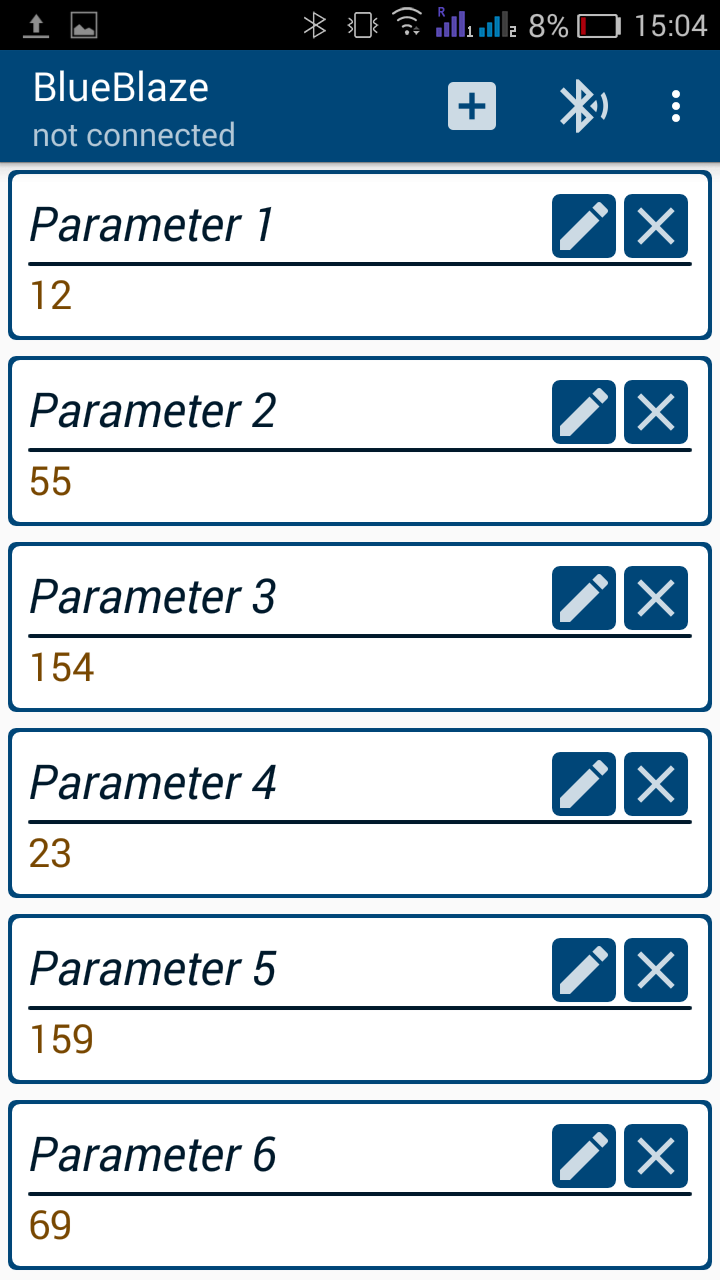
\includegraphics[scale=0.4]{images/Screenshot_itemlist.png}}
	\caption{Parameter List View}
	\label{fig:param-list}
\end{figure}

After launching the app Android OS creates main activity of the app. Main activity connects to the local database and retrieves if data present. After fetching data it renders views for each and display them on list view. If user wants to add a new parameter, plus button located on the toolbar provides this functionality. (See Figure \ref{fig:param-add})

\begin{figure}
	\centering
	\frame{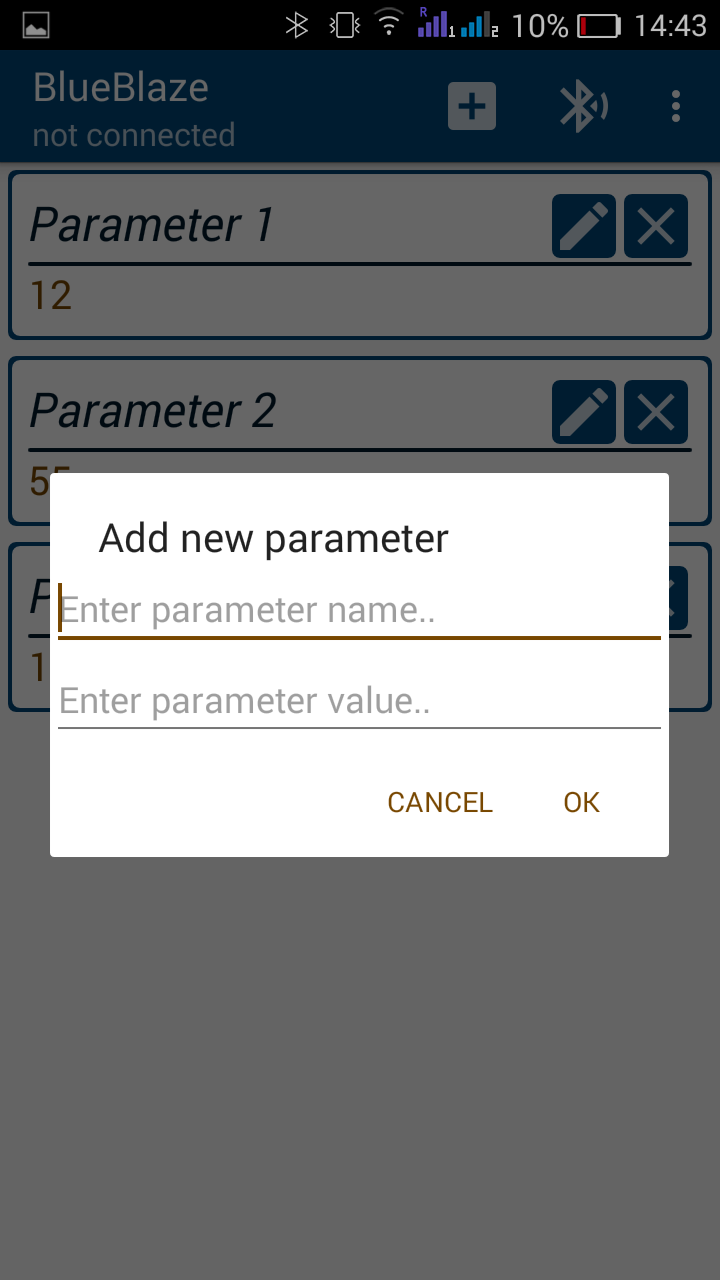
\includegraphics[scale=0.4]{images/Screenshot_add_parameter.png}}
	\caption{Parameter Add View}
	\label{fig:param-add}
\end{figure}

Edit and remove buttons are bundled together with the parameters to provide and intuitive user experience. Behaviour of these buttons are rather straightforward; edit button launches a fragment to edit the parameter (See Figure \ref{fig:param-edit}) and remove button removes parameter from the screen and the database.

\begin{figure}
	\centering
	\frame{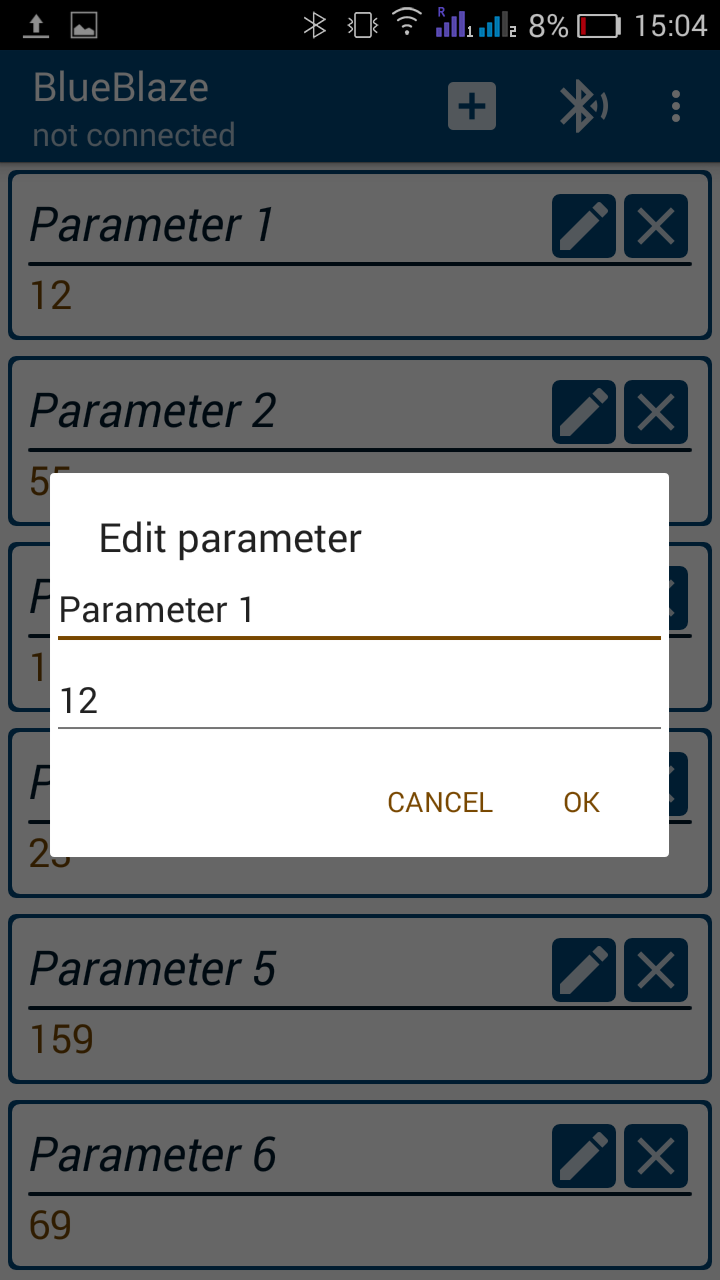
\includegraphics[scale=0.4]{images/Screenshot_edit_dialog.png}}
	\caption{Parameter Edit View}
	\label{fig:param-edit}
\end{figure}
 
Bluetooth button on the toolbar launches a different activity which is responsible for management of Bluetooth functionalities. Here nearby bluetooth devices can be scanned and paired or connection to previously paired devices can be established. (See Figure \ref{fig:bluetooth-menu})

\begin{figure}
	\centering
	\frame{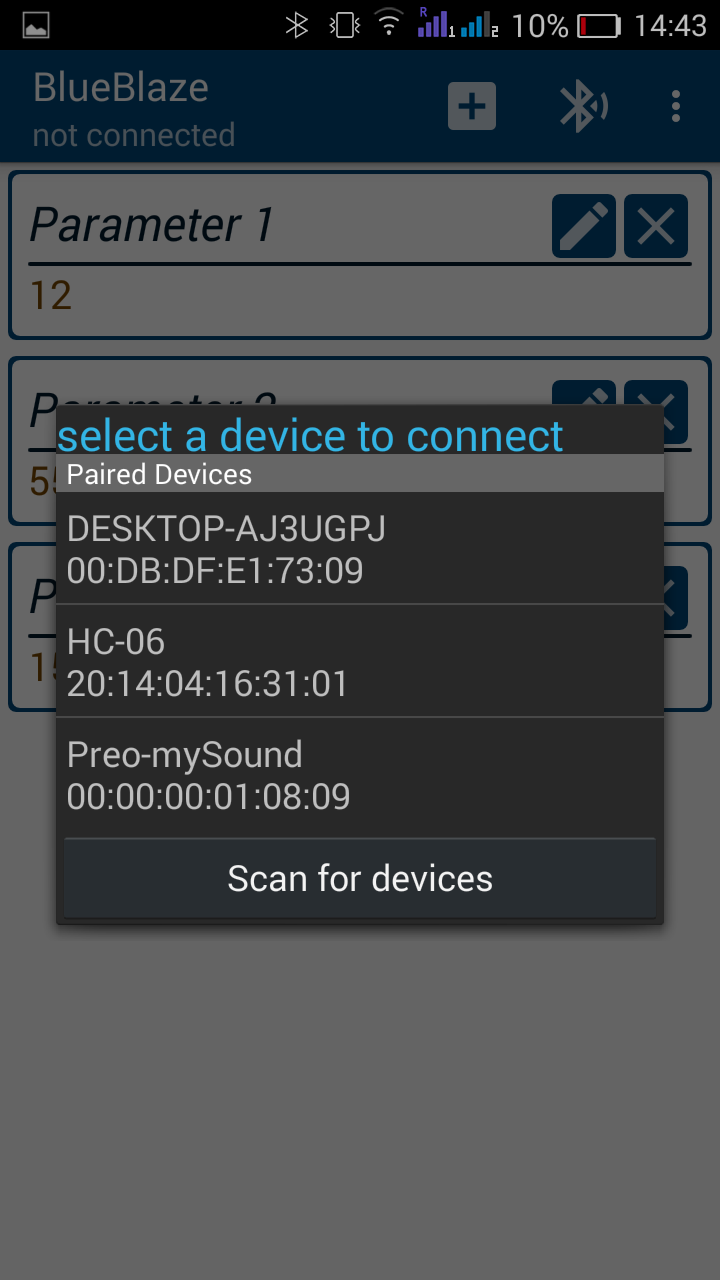
\includegraphics[scale=0.4]{images/Screenshot_bluetooth_menu.png}}
	\caption{Parameter Edit View}
	\label{fig:bluetooth-menu}
\end{figure}

Options menu is located on the upper right corner of the screen (See Figure \ref{fig:options-menu}). It provides buttons to access more functionality provided by the app. Exit button shuts down the app gracefully and makes it possible for Android OS to release allocated memory. Console button opens up a chat like view where it is possible exchange data with the connected device, however it should be noted this mode is unmanaged and merely provided to enable future extensions. Sync button sends the parameters stored in the database through the bluetooth connection to the target device. Insecure connection is provided here and it is optional to use. Device is also can be made discoverable by using "Make Discoverable" option.

\begin{figure}
	\centering
	\frame{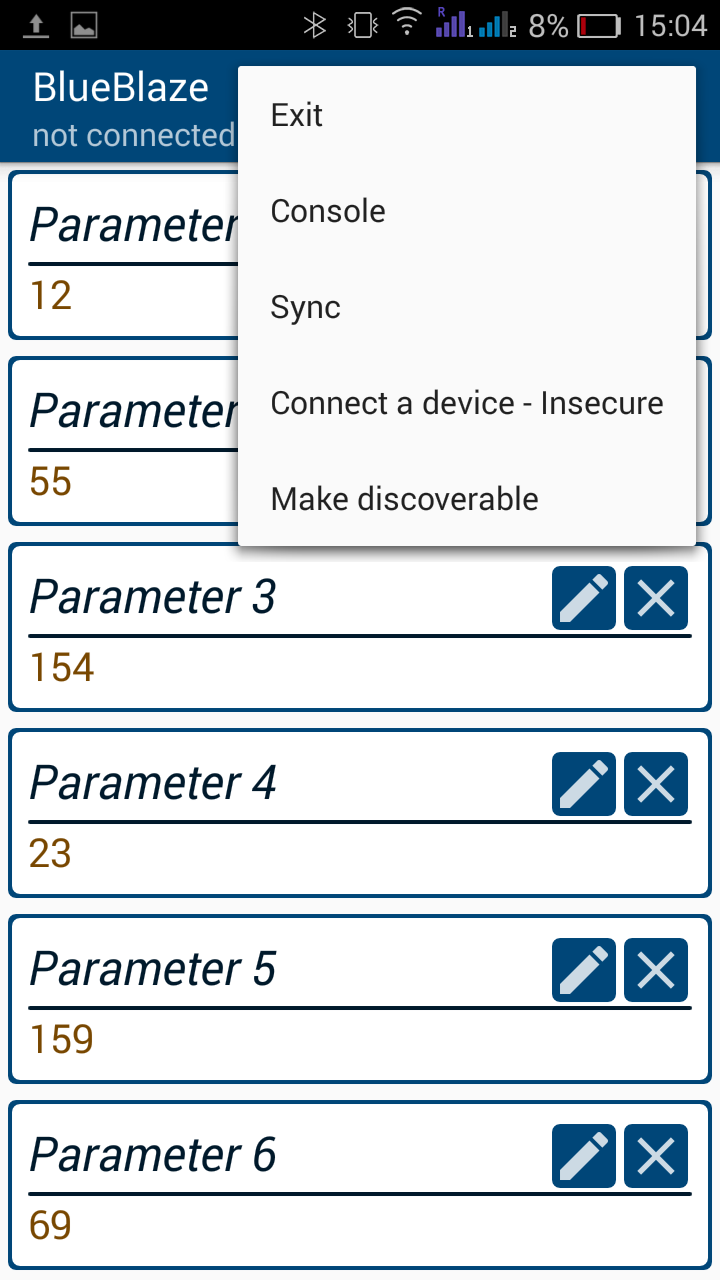
\includegraphics[scale=0.4]{images/Screenshot_options_menu.png}}
	\caption{Parameter Edit View}
	\label{fig:options-menu}
\end{figure}

\section{Bluetooth}

Bluetooth related functionalities implemented as a service for the rest of the application. In any given moment service can have one of four states. 

These states are :
\begin{itemize}
	\item STATE\_NONE		: Idle state
	\item STATE\_LISTEN		: Listening for incoming connections
	\item STATE\_CONNECTING	: Initiating an outgoing connection
	\item STATE\_CONNECTED	: Connected to a remote device
\end{itemize}

Bluetooth service operates with separate threads and it does not block main thread of the application. It holds a reference to main thread and when a connection gets accepted or data transfer takes place it calls callback handler of main thread. 
Android SDK bluetooth libraries utilised for the implementation of this service. As a basis, example provided by Google \cite{google-bluetooth} used and it is extended for the purposes of this application.

\section{Database}
Saving and restoring data provided by the user is needed for application, for this purpose a database is implemented with the app. SQLite \cite{google-sqlite} is provided with Android SDK and it can be used with great ease.

Database is created during the installation of the app and tables are also created inside the database at this moment. Database has one table which holds the parameters entered by the user. It has following columns :

\begin{itemize}
	\item ID		: Auto generated id 
	\item NAME		: Name of the parameter
	\item VALUE		: Value of the parameter
\end{itemize}

A Wrapper code is developed for the database operations as an abstraction layer. This layer is consumed by the rest of the application whenever a parameter created, edited or removed. 

\section{Usage}

Upon launching BlueBlaze app for the first time, it checks the database and displays available data. If no data present it displays an empty screen. Here user can add parameters using add button on the toolbar. After adding the parameters they can be sent to paired bluetooth device using sync button on options menu. It should be noted if there is no connection, app informs user on lack of connection. 











